\documentclass[10pt,aspectratio=149]{beamer}
\usecolortheme{Calm}
\usetheme{Calm}
%\usefonttheme[onlymath]{serif} % beamer force les maths en cmss par défaut, qui n'a pas de vrai gras : \mathbf{} restait fin
\usepackage{amsmath}
\usepackage{pgfplots}
\pgfplotsset{compat=1.18}
\usepackage{pgfplotstable}
\usepackage[utf8]{inputenc}
\usepackage{hyperref}
\RequirePackage[absolute,overlay]{textpos}
%\usepackage[sfdefault]{cabin}
%\usepackage[T1]{fontenc}
%\setlength{\TPHo{}rizModule}{\paperwidth}
%\setlength{\TPVertModule}{\paperheight}
%\definecolor{OQEdarkblue}{HTML}{046085}


\defbeamertemplate*{background canvas}{bg}
{%
  \color{lightgray!40}\vrule width\paperwidth height\paperheight% added bg color
}

% Centered, larger display equation
\newcommand{\keyeq}[1]{%
  \begin{center}
    \Large$\displaystyle #1$
  \end{center}%
}

% Same style, for a system of equations aligned on "="
% (rows separated by \\, each row written as LHS &= RHS)
\newcommand{\keyeqs}[1]{%
  \begin{center}
    \normalsize$\displaystyle
    \begin{aligned}
    #1
    \end{aligned}
    $
  \end{center}%
}

%------------------------------

\author{Dominique Gravel}
\title{Realistic landscapes}
\date{August 25th, 2026}
\institute{Université de Sherbrooke \\ Summer school in biodiversity modelling}

%------------------------------
% TITLE SLIDE
%------------------------------

\usebackgroundtemplate
{
  
\includegraphics[width=\paperwidth,height=\paperheight]{bg}%
}

\begin{document}

	\begin{frame}[plain]
		\titlepage
	\end{frame}

%------------------------------

{
\usebackgroundtemplate{}
\begin{frame}

	\pagecolor{BDQC1st}
	\color{white}

	\LARGE{\textit{Exercise}}

\end{frame}
}

%------------------------------

\begin{frame}{30-30 Target}

    \begin{center}
        
\includegraphics[height=0.7\textheight]{Figs/appel}\\
    \end{center}

\end{frame}

%------------------------------

\begin{frame}[fragile]{30-30 Target}

    \begin{itemize}
        \item Southern Québec has a deficit of protected areas
        \item Mostly small private areas
        \item Few large tracts of public lands 
    \end{itemize}

   Based on metapopulation theory, should we aim at protecting as many private lands as possible, or should we put our efforts on public lands ?

\end{frame}

%------------------------------

{
\usebackgroundtemplate{}
\begin{frame}

	\pagecolor{BDQC1st}
	\color{white}

	\LARGE{\textit{Theory}}

\end{frame}
}

%------------------------------

\begin{frame}{Spatially explicit metapopulation dynamics}

	Each patch $x$ is unique. We therefore need to track the probability it is occupied : 

    \keyeq{\frac{dp_x}{dt} = c_x P_x(1-p_x) - e_xp_x}
    
    Note the difference in colonization, $P_x$ is the total amount of propagules reaching patch $x$. We will define this quantity in a few slides. 

\end{frame}

%------------------------------

\begin{frame}{What makes a patch unique ?}


\end{frame}

%------------------------------

\begin{frame}{What makes a patch unique ?}

    \begin{itemize}
        \item The quality of the environment
        \item The amount of propagules it produces
        \item Spatial location 
        \item Local extinction probability 
    \end{itemize}

\end{frame}

%------------------------------

\begin{frame}{What makes a patch unique ?}{Area}

    Population theory has established that extinction probability from demographic stochasticity $e \propto A^{-1}$

    A first modification of the Levins model is therefore : 

    \keyeq{extinction = \frac{e_x}{A_x}p_x}

    where $e_x$ could vary locally because of its intrinsic quality

\end{frame}

%------------------------------

\begin{frame}{What makes a patch unique ?}{Location}

	\begin{columns}
		\begin{column}{0.5\textwidth}
            \begin{itemize}
                \item Distance to neighbours
                \item State of neighbours
                \item Area of neigbhours
            \end{itemize}
		\end{column}
%----
		\begin{column}{0.5\textwidth}
            \begin{center}
                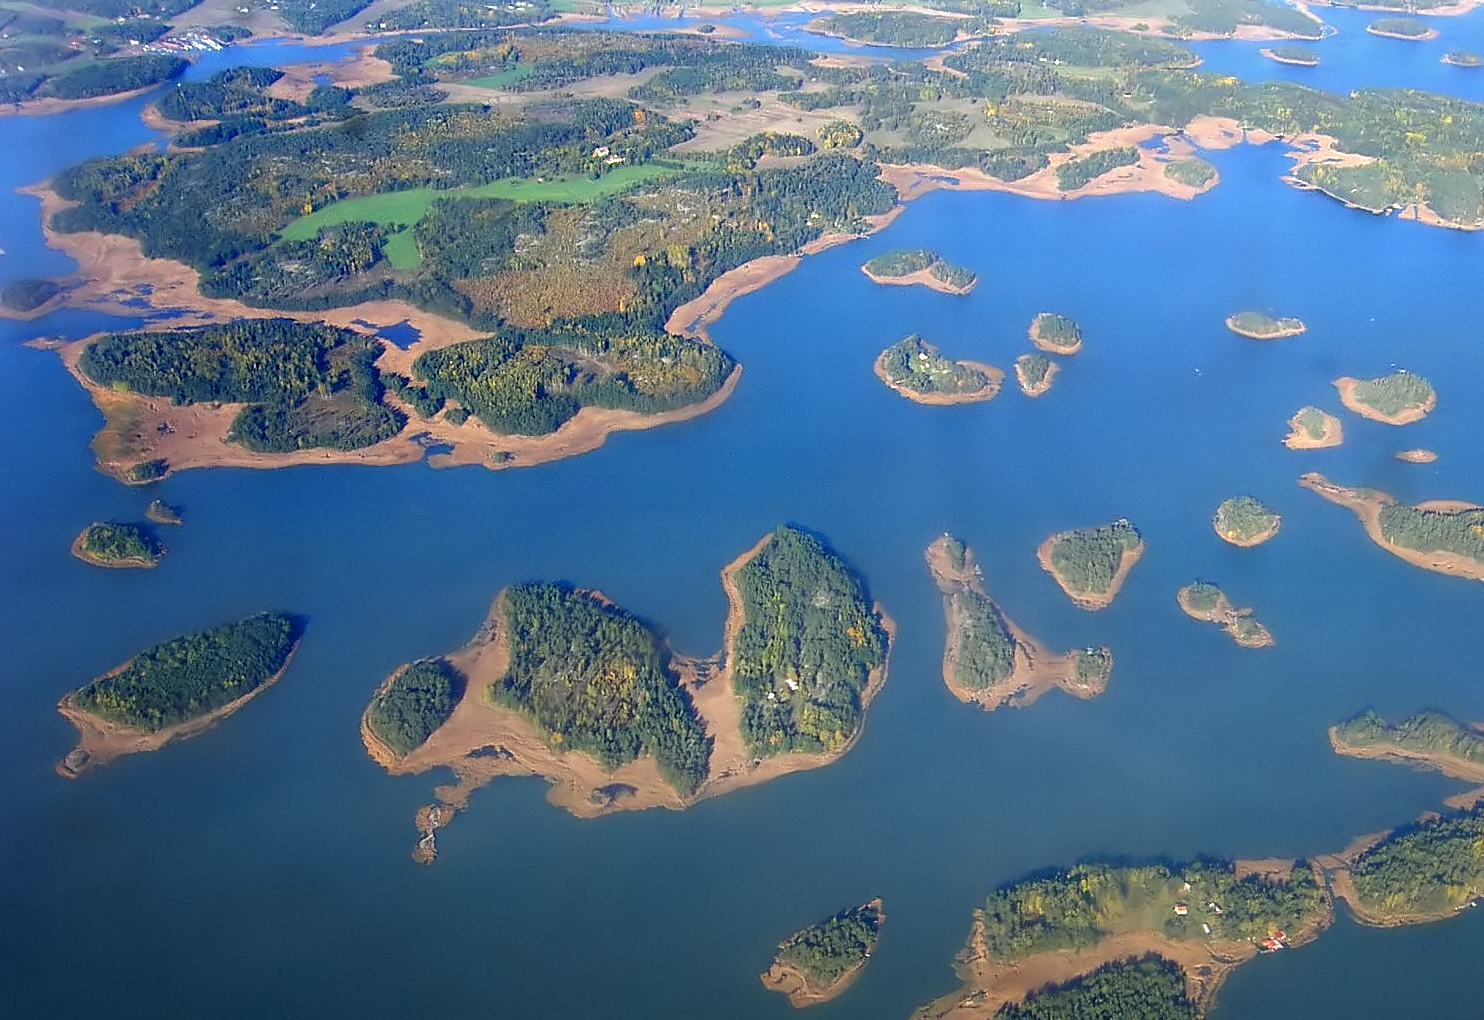
\includegraphics[height=0.4\textheight]{Figs/archipelago} 
            \end{center}
		\end{column}
	\end{columns}

\end{frame}

%------------------------------

\begin{frame}{What makes a patch unique ?}{Dispersal kernel}

	Propagules are more likely to reach nearby sites than distant ones. The minimal model for this hypothesis is the exponential function of distance :

    \keyeq{K(x,y)=exp(-\alpha d_{xy})}

    where $\alpha^{-1}$ is the average dispersal distance $d_{xy}$

\end{frame}

%------------------------------

\begin{frame}{What makes a patch unique ?}{Total dispersal}

	Now we need to aggregate dispersal from all neighbours. A first (wrong - but very common) approximation is : 
    
       \keyeq{P_x = \sum_{x\neq y}^N K(x,y)p_yA_y}
    
    1st note : it's the size of the patch producing propagules, not the one receiving propagules, that is size dependent.

    2nd note : this formulation is not exact because it assumes that only one colonization occurs per unit time. It's however practicle because it remains linear

\end{frame}

%------------------------------

\begin{frame}{Spatially explicit metapopulation dynamics}{Full picture}

	Plugging these definitions into the main equation we get : 

    \keyeq{\frac{dp_x}{dt} = c_x \sum_{x\neq y}^N K(x,y)p_yA_y (1-p_x) - \frac{e_x}{A_x}p_x}
    
    For now we will consider parameters $c$ and $e$ to be constant across all locations (we'll get back to it at the end). 

\end{frame}

%------------------------------

\begin{frame}{A compact notation}

	We can re-organize the equation using matrix notation. 

    Define : 

    \keyeq{m_{xy} = K(x,y)A_xA_y}

    where $m_{xy}$ is the value in the entry $[x,y]$ of matrix $\mathbf{M}$. 

    \vskip 1em

    Matrix $\mathbf{M}$ therefore contains information on the spatial location of all patches, their contribution to colonization as well as the effect of area on extinction probability. All elements on the diagonal are set to 0. 

\end{frame}

%------------------------------

\begin{frame}{For a simple solution}

	After a bit of magic (See Ovaskainen and Hanski 2002 for the maths), we find the very elegant condition for persistence :  

    \keyeq{\lambda_M > \frac{e}{c}}

    where $\lambda_M$ is the first eigenvalue of the matrix $\mathbf{M}$. A weighted average of the equilibrium vector of occupancies is : 

    \keyeq{p^* = 1 - \frac{1}{\lambda_M}\frac{e}{c}}

\end{frame}

%------------------------------

\begin{frame}{Back to SLOSS}

    We now have a fairly simple tool to check the effect of patch size distribution on metapopulation persistence. 

    Two phenomenon happen at the same time for a constant total surface : 

    \begin{enumerate}
        \item Larger patches have lower extinction probability and larger propagule production
        \item Distance between patches increases as the number of patches decreases
    \end{enumerate}

\end{frame}

%------------------------------

\begin{frame}{Back to SLOSS}{Examples}

    \begin{center}
        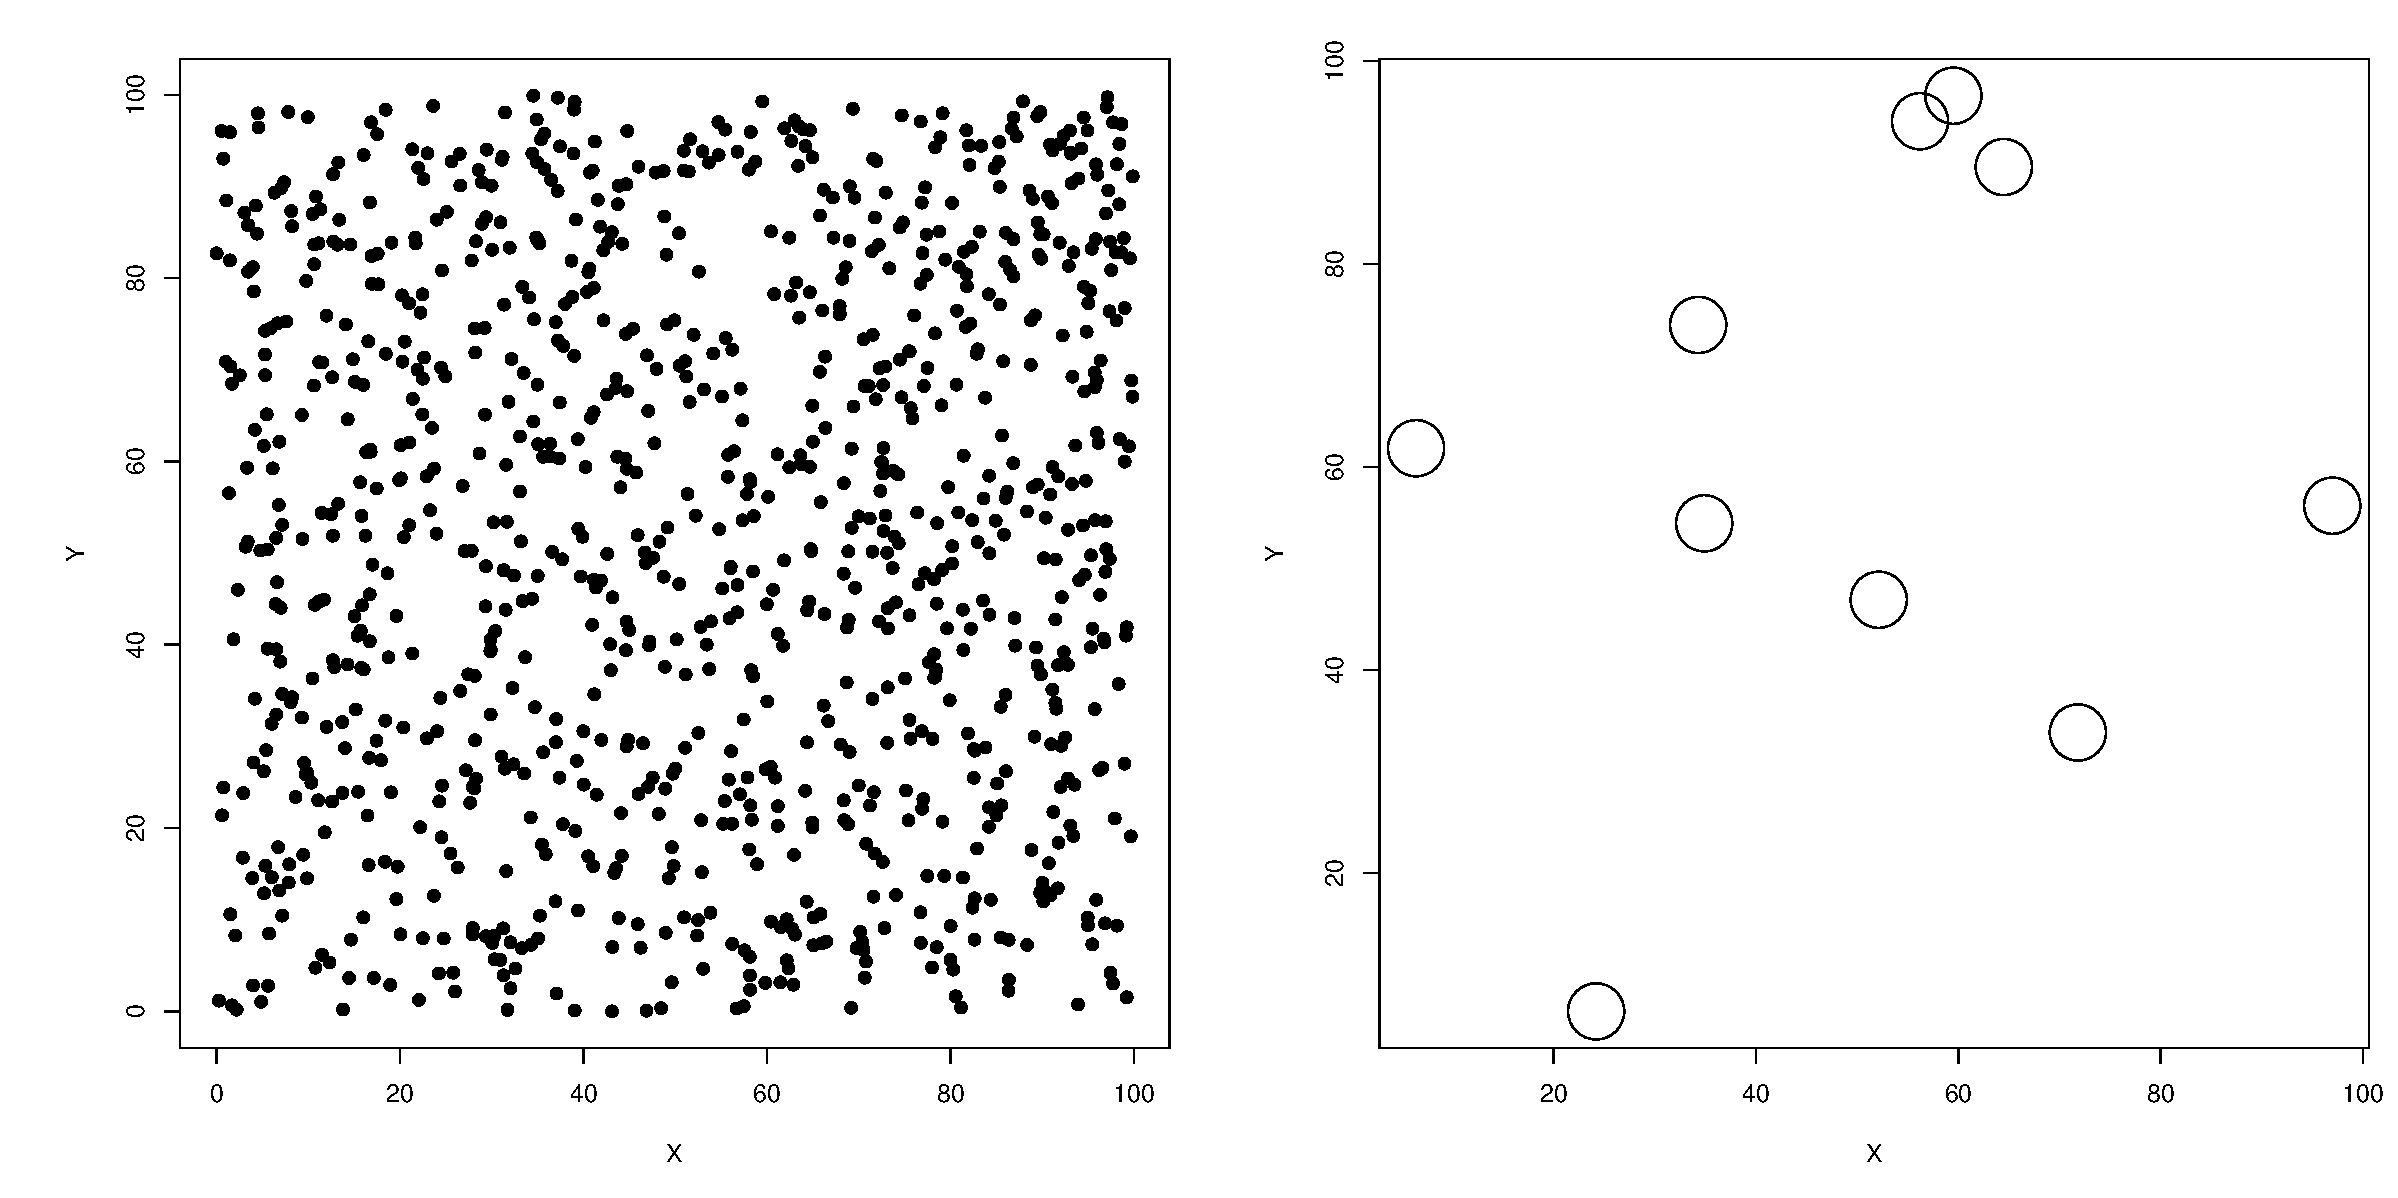
\includegraphics[height=0.5\textheight]{Figs/figure1}\\           
    \end{center}

\end{frame}

%------------------------------

\begin{frame}{Back to SLOSS}{Examples}

    \begin{center}
        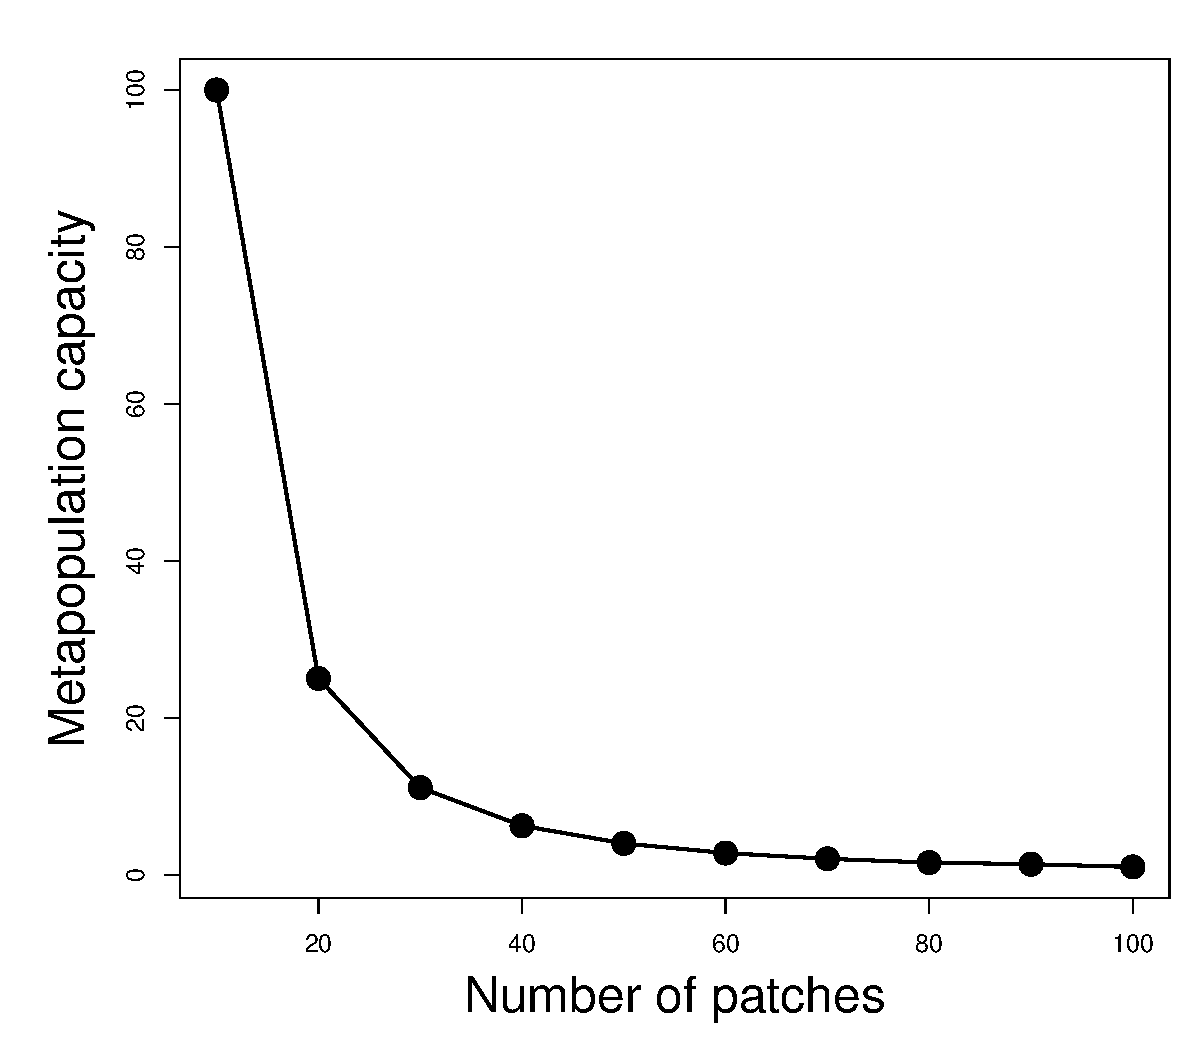
\includegraphics[height=0.5\textheight]{Figs/figure2}\\           
    \end{center}

    Note : the basic model assumes a certain effect of patch area on metapopulation dynamics. It is possible to modify it with $A^\gamma$ where $\gamma$ is a tuning parameter. 

\end{frame}

%------------------------------

\begin{frame}{Still an open debate}

    \begin{center}
        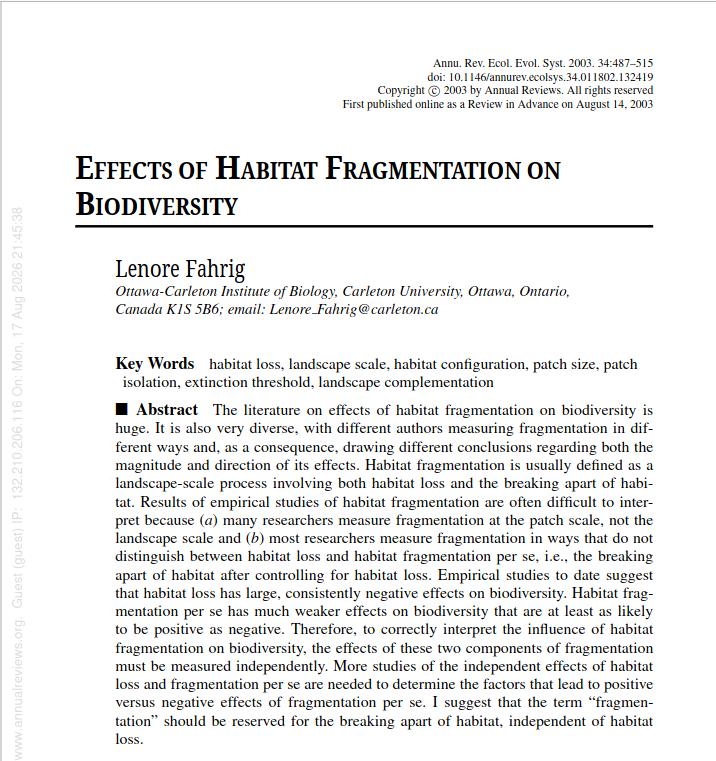
\includegraphics[height=0.7\textheight]{Figs/fahrig2003}\\
    \end{center}

\end{frame}

%------------------------------

{
\usebackgroundtemplate{}
\begin{frame}

	\pagecolor{BDQC1st}
	\color{white}

	\LARGE{\textit{And what about patch quality ?}}

\end{frame}
}

%------------------------------

\begin{frame}{Expected future distribution}
    \begin{columns}
       \begin{column}{0.5\textwidth}
          \begin{center}
             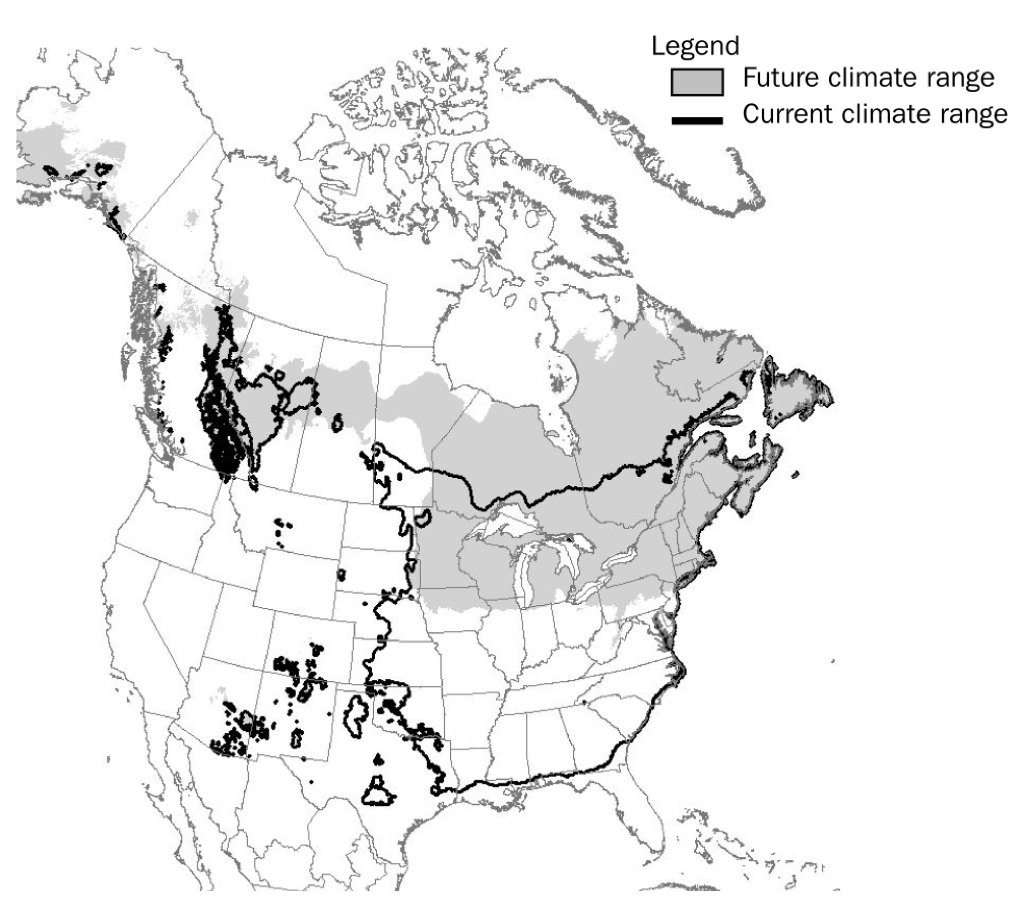
\includegraphics[height=0.5\textheight]{Figs/mckenney}\\
             McKenney et al. 2007. Bioscience
          \end{center}
       \end{column}
%----
       \begin{column}{0.5\textwidth}
          \begin{itemize}    
             \item Phenomenological;
             \item No demography;
             \item No biotic interactions;
             \item No dispersal limitations;
             \item Equilibrium distribution;        
          \end{itemize}
       \end{column}
    \end{columns}        
 \end{frame}

%------------------------------

\begin{frame}{Non-linear transitions}
    \begin{center}
       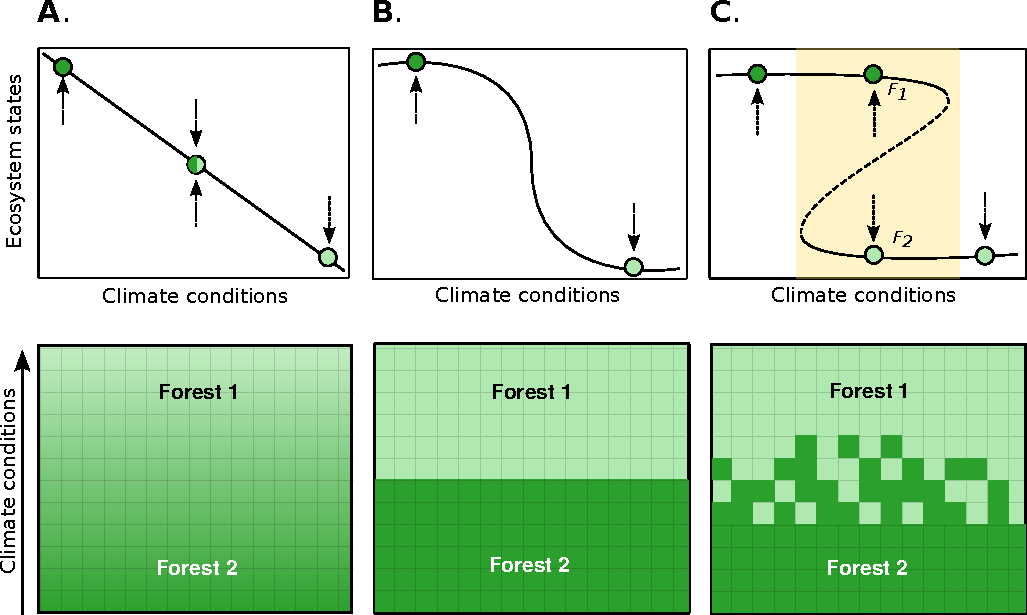
\includegraphics[height=0.6\textheight]{Figs/states}\\
    \end{center}
 \end{frame}

%-------------------------------------------------------------------------------

 \begin{frame}{Critical slowing down}
    \begin{center}
       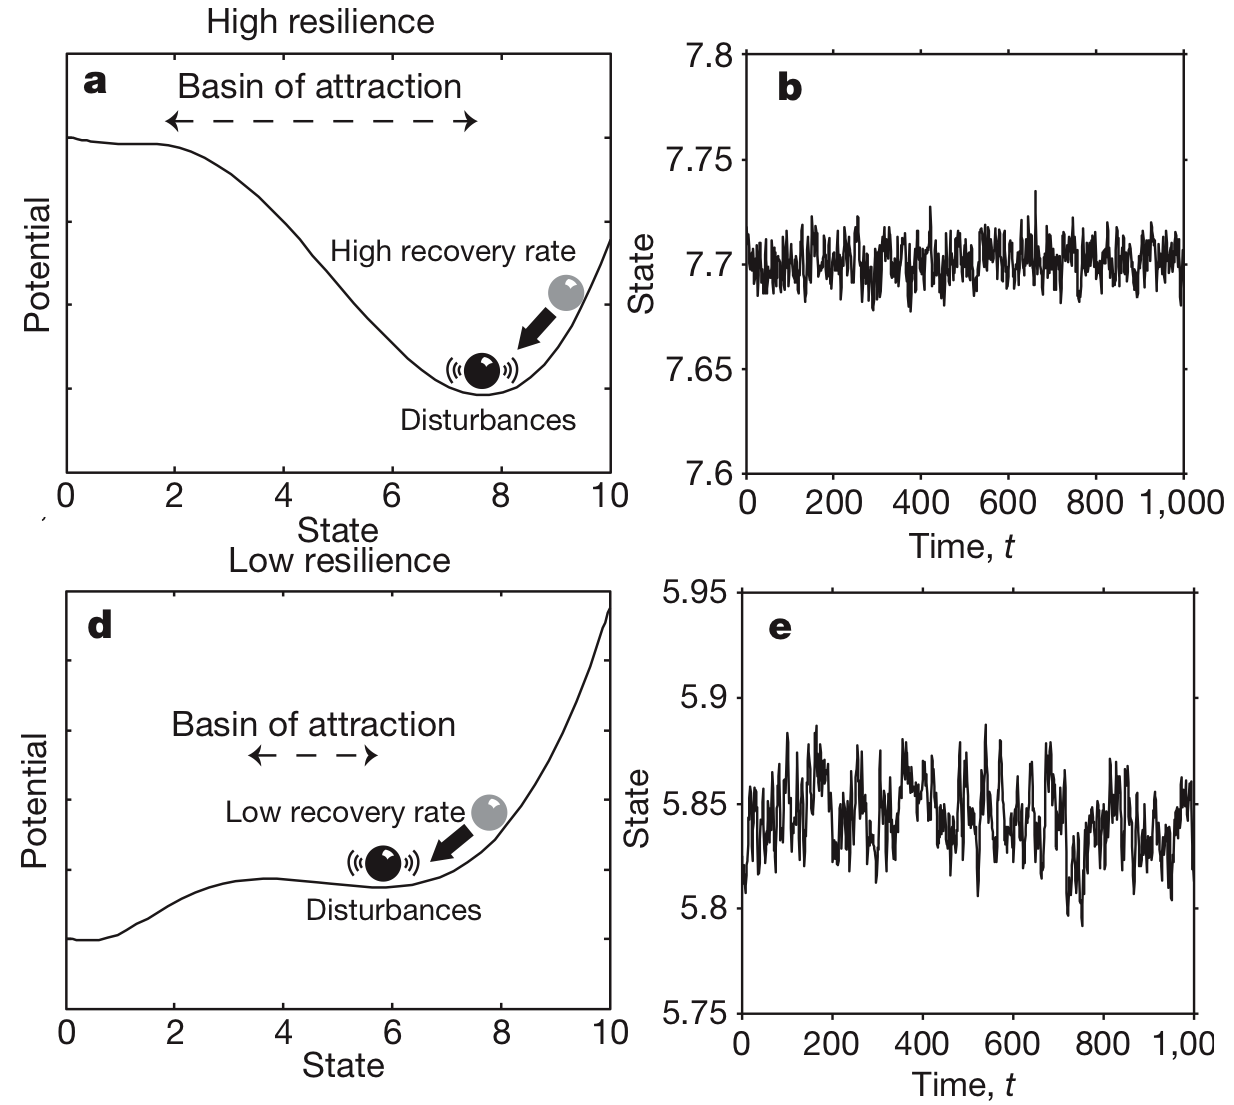
\includegraphics[height=0.6\textheight]{Figs/early_warnings}\\
       Scheffer et al. (2009) Nature.
    \end{center}
 \end{frame}

%-------------------------------------------------------------------------------

\begin{frame}{Model for range limits}
    Metapopulation dynamics: \\
 
    \keyeq{\frac{dp(E)}{dt} = \underbrace{c(E)p(E)(h(E) - p(E))}_{\mbox{Colonisation}} - \underbrace{e(E)p(E)}_{\mbox{Extinction}}}
    \vskip 1em
 
    Which yields the equilibrium distribution:\\  
    \keyeq{\overline{p}(E) = h(E) - \frac{e(E)}{c(E)}}
 
    \end{frame}
 
 %-------------------------------------------------------------------------------
 
    \begin{frame}{Model for range limits}{Amount of change}
    
    The sensitivity of the system to a changing environment is thus given by: \\
 
    \keyeq{\frac{\partial \overline{p}(E)}{\partial E}}
 
    \end{frame}
 
 %------------------------------------------------------------------------------
 
    \begin{frame}{Asymptotic rate of convergence}
    
    Consider a small deviation to the equilibrium under the new environmental conditions, $E_1$, called $\delta$: \\
 
    \keyeq{\frac{d(\overline{p}(E_1) + \delta)}{dt} = \frac{d\overline{p}(E_1)}{dt} + \frac{d\delta}{dt}}
 
    \vskip 1em
    With: \\
    \keyeq{\delta = \frac{\partial \overline{p}(E_1)}{\partial E}}
 
    \vskip 1em
    Linearization of the system around this equilibrum gives the dynamics of the small deviation (the leading eigenvalue in thecase of a system of equations).
 
    \end{frame}
 
 %-------------------------------------------------------------------------------
 
    \begin{frame}{Asymptotic rate of convergence}{Metapopulation}
    
    Within the range limit: \\
 
    \keyeq{\lambda = e(E) - c(E)}
    
    Outside the range limit: 
 
    \keyeq{\lambda = c(E) - e(E)}
 
    A the range limit: 
 
    \keyeq{\lambda = c(E) - e(E) = 0}
 
    \end{frame}
 
 %-------------------------------------------------------------------------------
 
 \begin{frame}{Data}
    \begin{columns}
       \begin{column}{0.5\textwidth}
          \begin{center}
             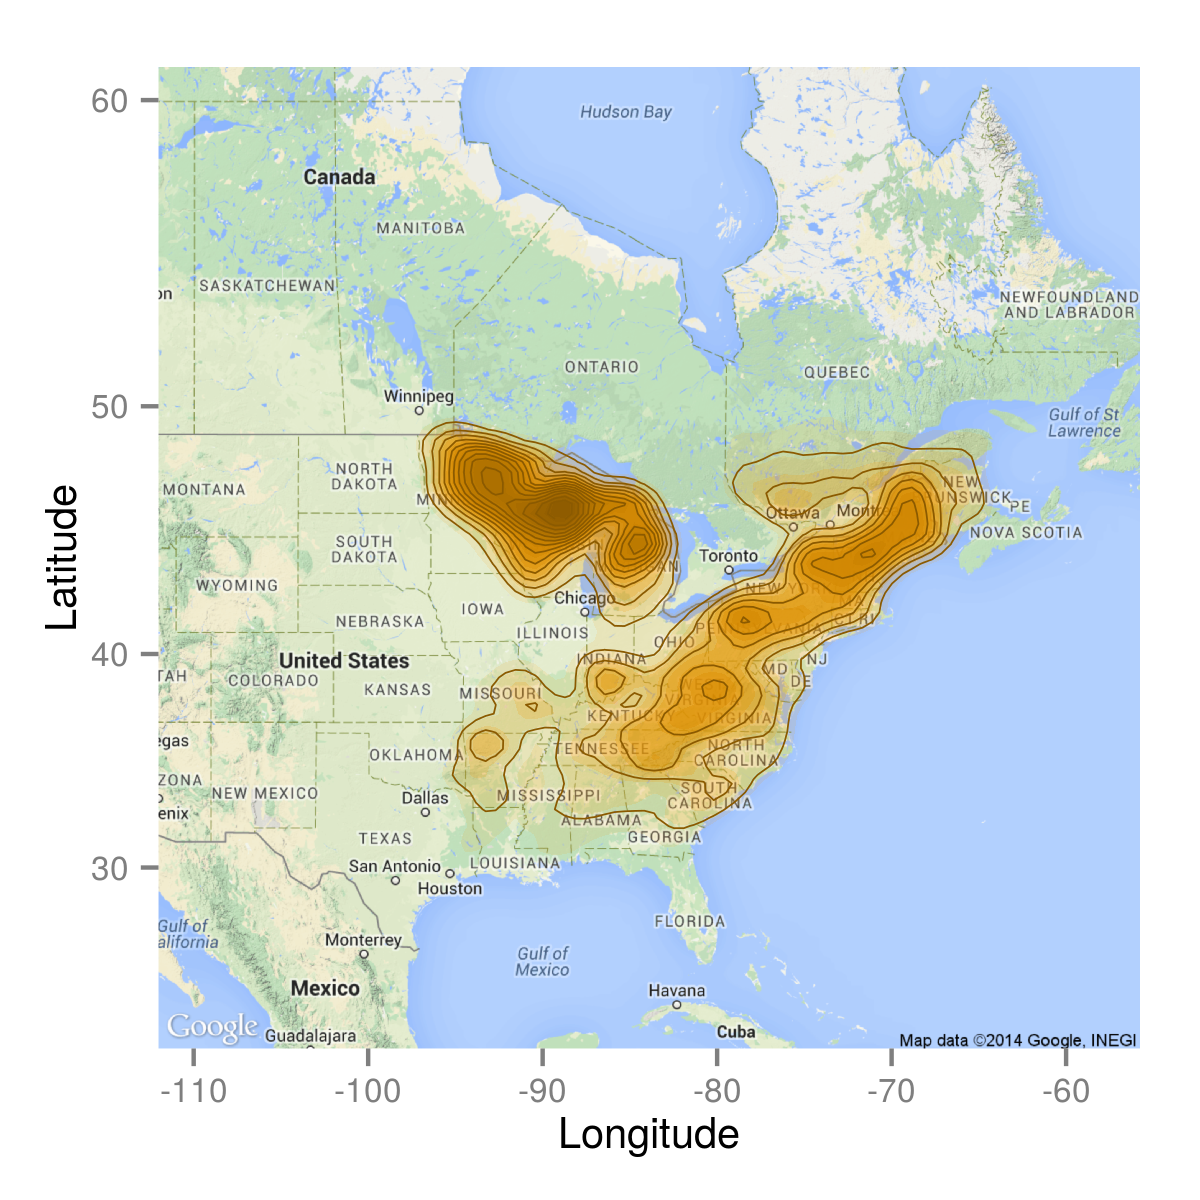
\includegraphics[height=0.6\textheight]{Figs/plots_map}
          \end{center}
       \end{column}
%----
       \begin{column}{0.5\textwidth}
           \begin{itemize}
             \item Permanent Forest Inventory plots from U.S. and Canada;
             \item Single tree measurements;
             \item 2-4 measurements;
             \item 5-15 years return interval;
             \item Classification in presence-absence;
          \end{itemize}
       \end{column}
    \end{columns}        
 \end{frame}   

%-------------------------------------------------------------------------------

 \begin{frame}{Fitting procedure}
    \begin{itemize}
       \item Colonization and extinction models;
       \item Each transition is a binomial model; 
       \item Approximation of the propagule pressure;
       \item Each transition is a function of annual average temperature and total precipitations;
       \item Bayesian parameter estimation with MCMC;
    \end{itemize}
 \end{frame}

%-------------------------------------------------------------------------------

\begin{frame}{Solving for range limits}
    \begin{center}
       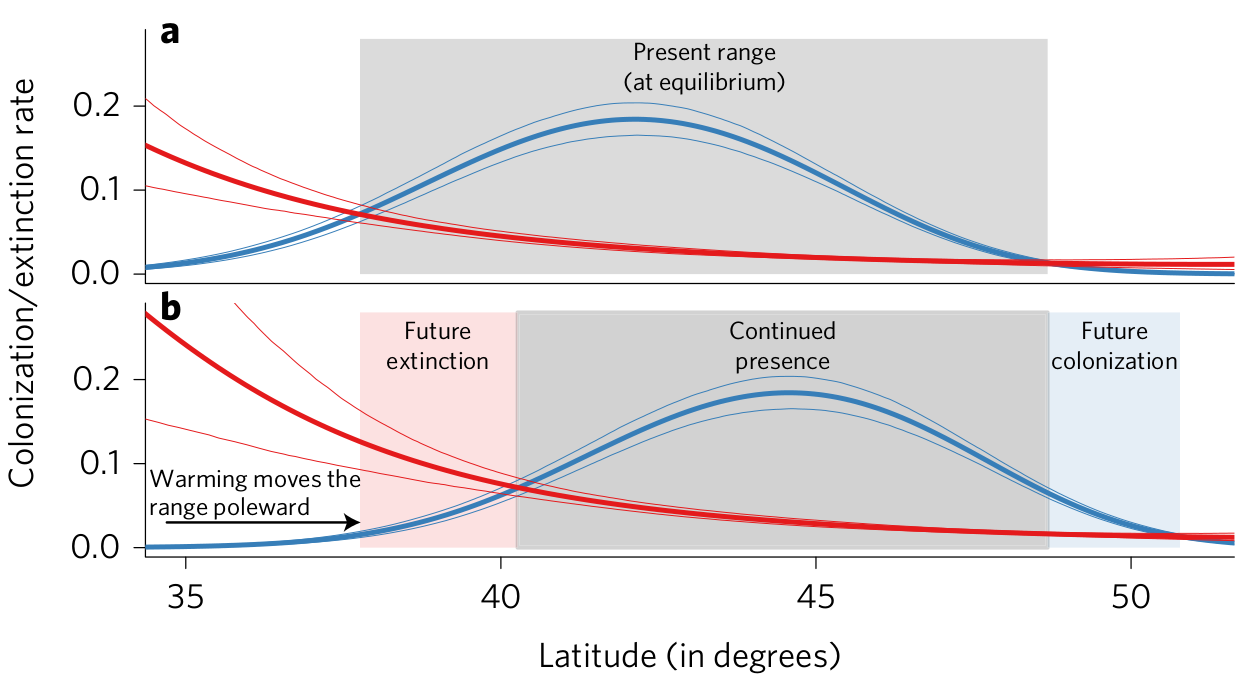
\includegraphics[height=0.5\textheight]{Figs/talluto1}\\
       \footnotesize{Talluto et al. 2017. Nature Ecology and Evolution}               
    \end{center}
 \end{frame}

%-------------------------------------------------------------------------------

  \begin{frame}{Solving for range limits}
   \begin{center}
       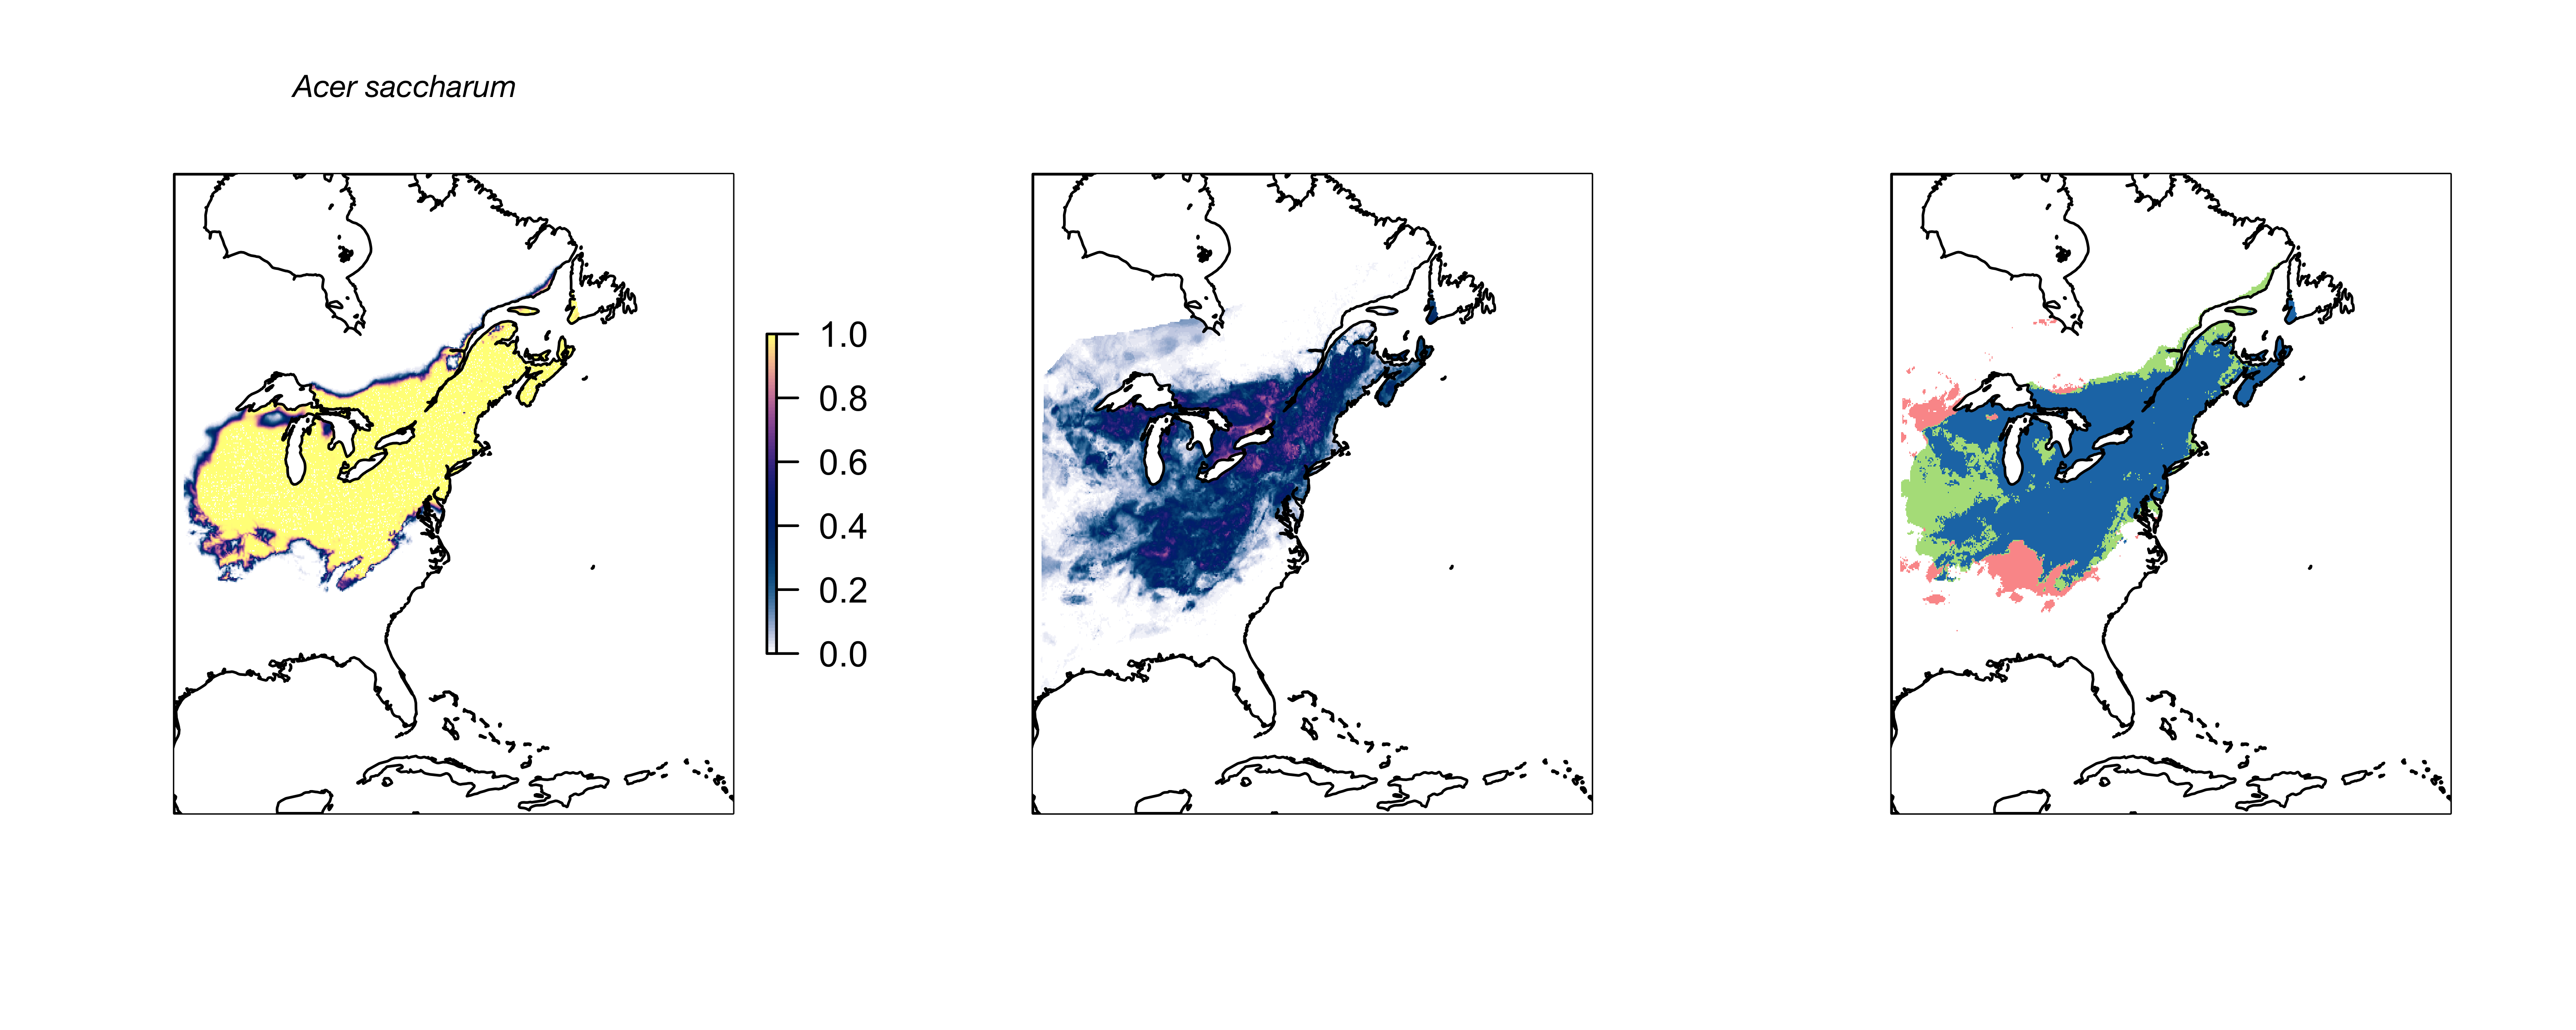
\includegraphics[height=0.55\textheight]{Figs/sugar_maple}\\
       \footnotesize{Talluto et al. 2017. Nature Ecology and Evolution} 
    \end{center}
 \end{frame}

%-------------------------------------------------------------------------------

\begin{frame}{Solving for range limits}
    \begin{center}
         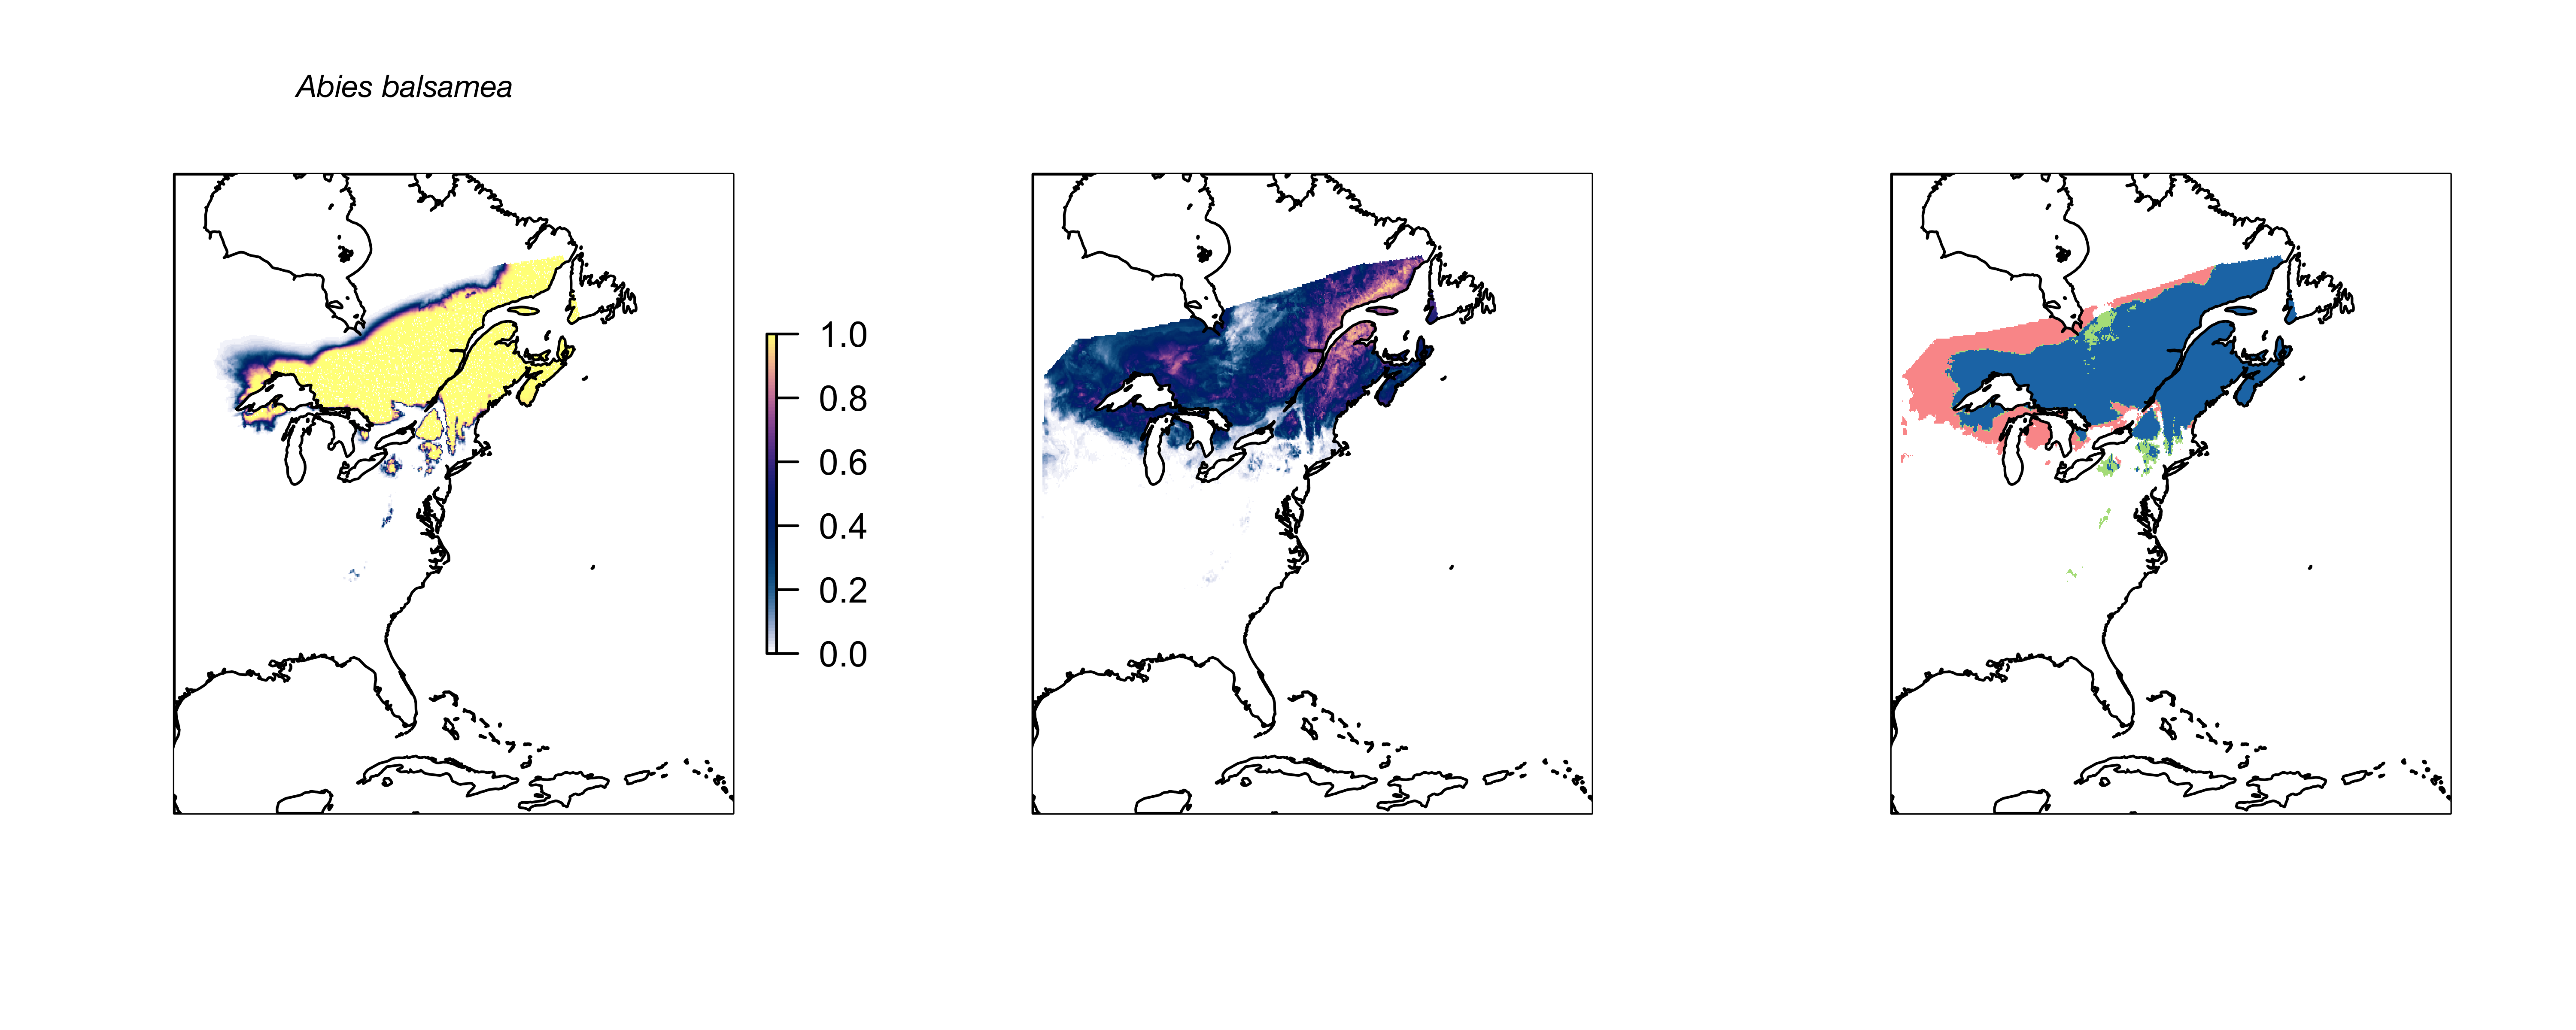
\includegraphics[height=0.55\textheight]{Figs/balsam_fir}\\
         \footnotesize{Talluto et al. 2017. Nature Ecology and Evolution} 
      \end{center}
   \end{frame}

%-------------------------------------------------------------------------------

\begin{frame}{Demography}
    \begin{center}
       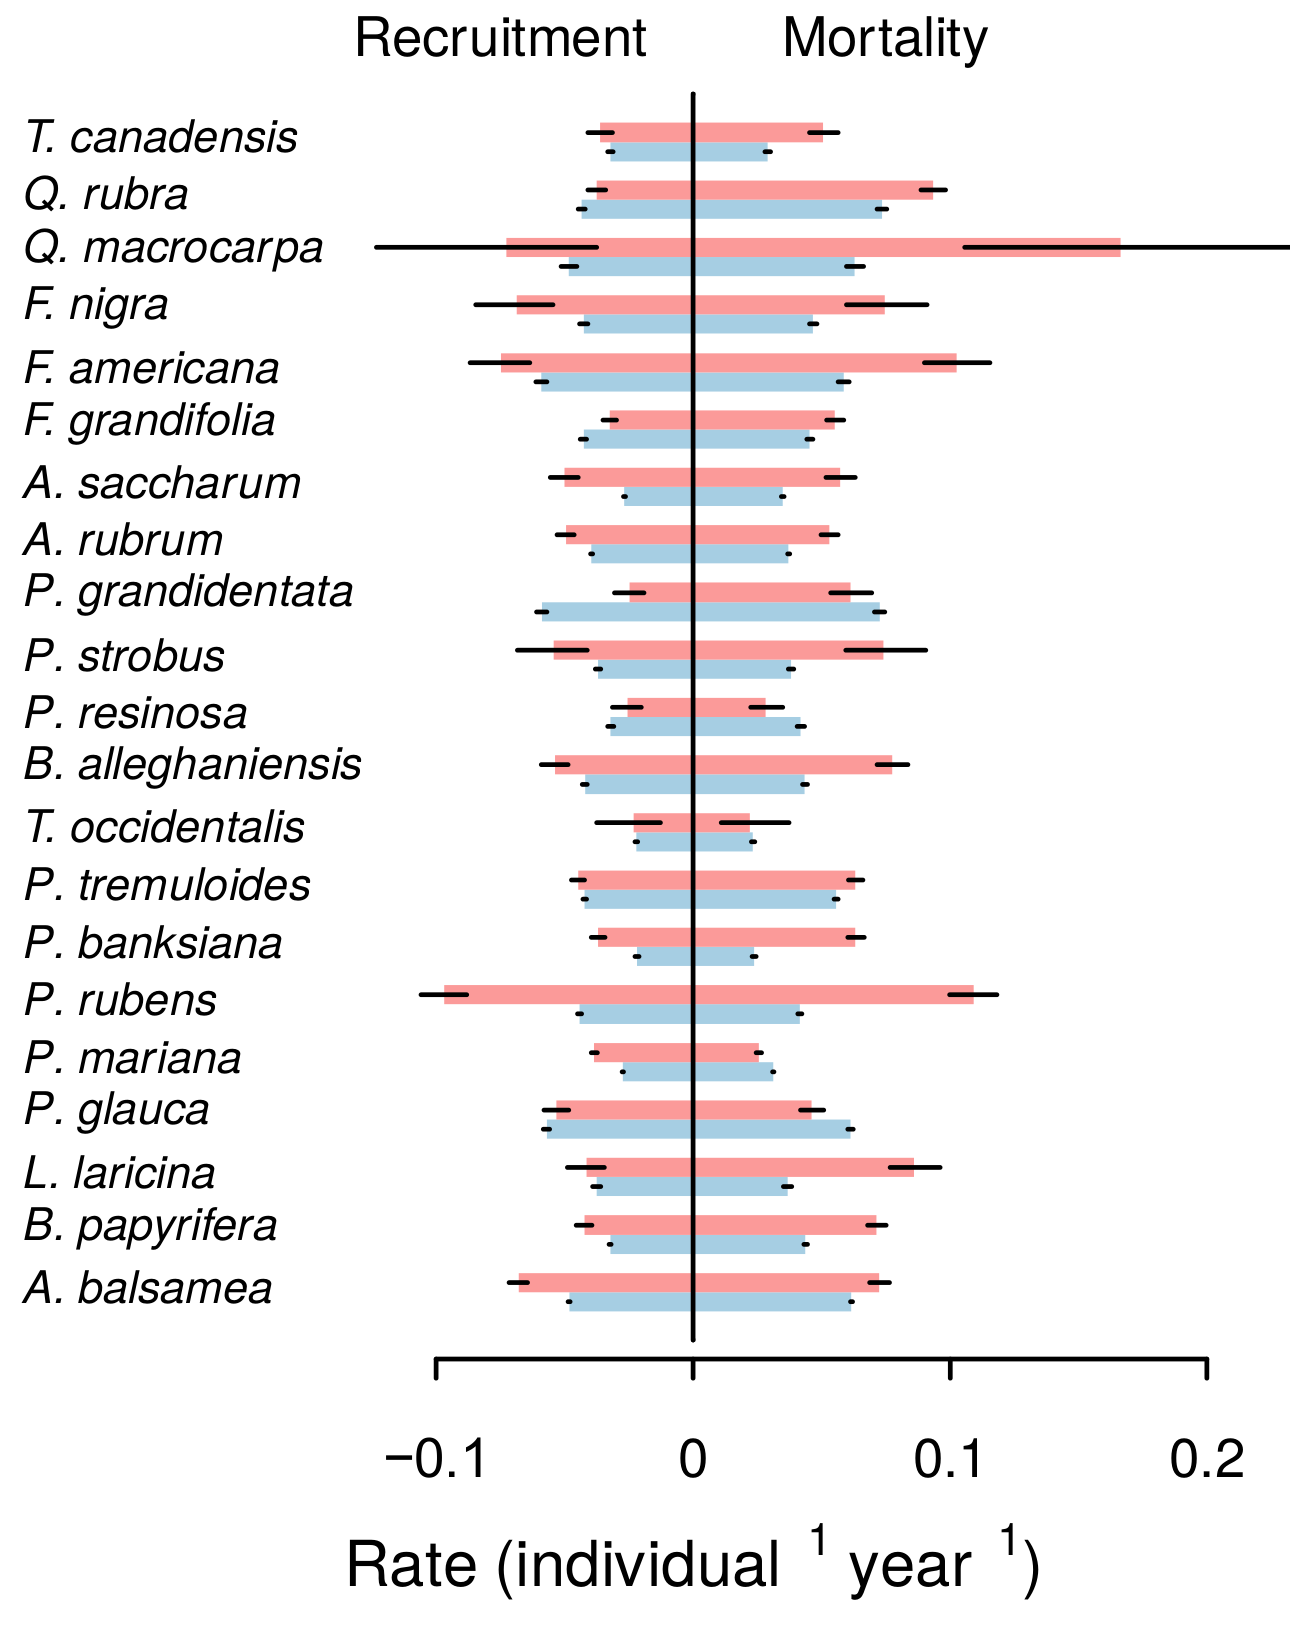
\includegraphics[height=0.6\textheight]{Figs/demography}\\
       \footnotesize{Talluto et al. 2017. Nature Ecology and Evolution} 
    \end{center}
 \end{frame}

%-------------------------------------------------------------------------------

\begin{frame}{Rate of response}
    \begin{center}
       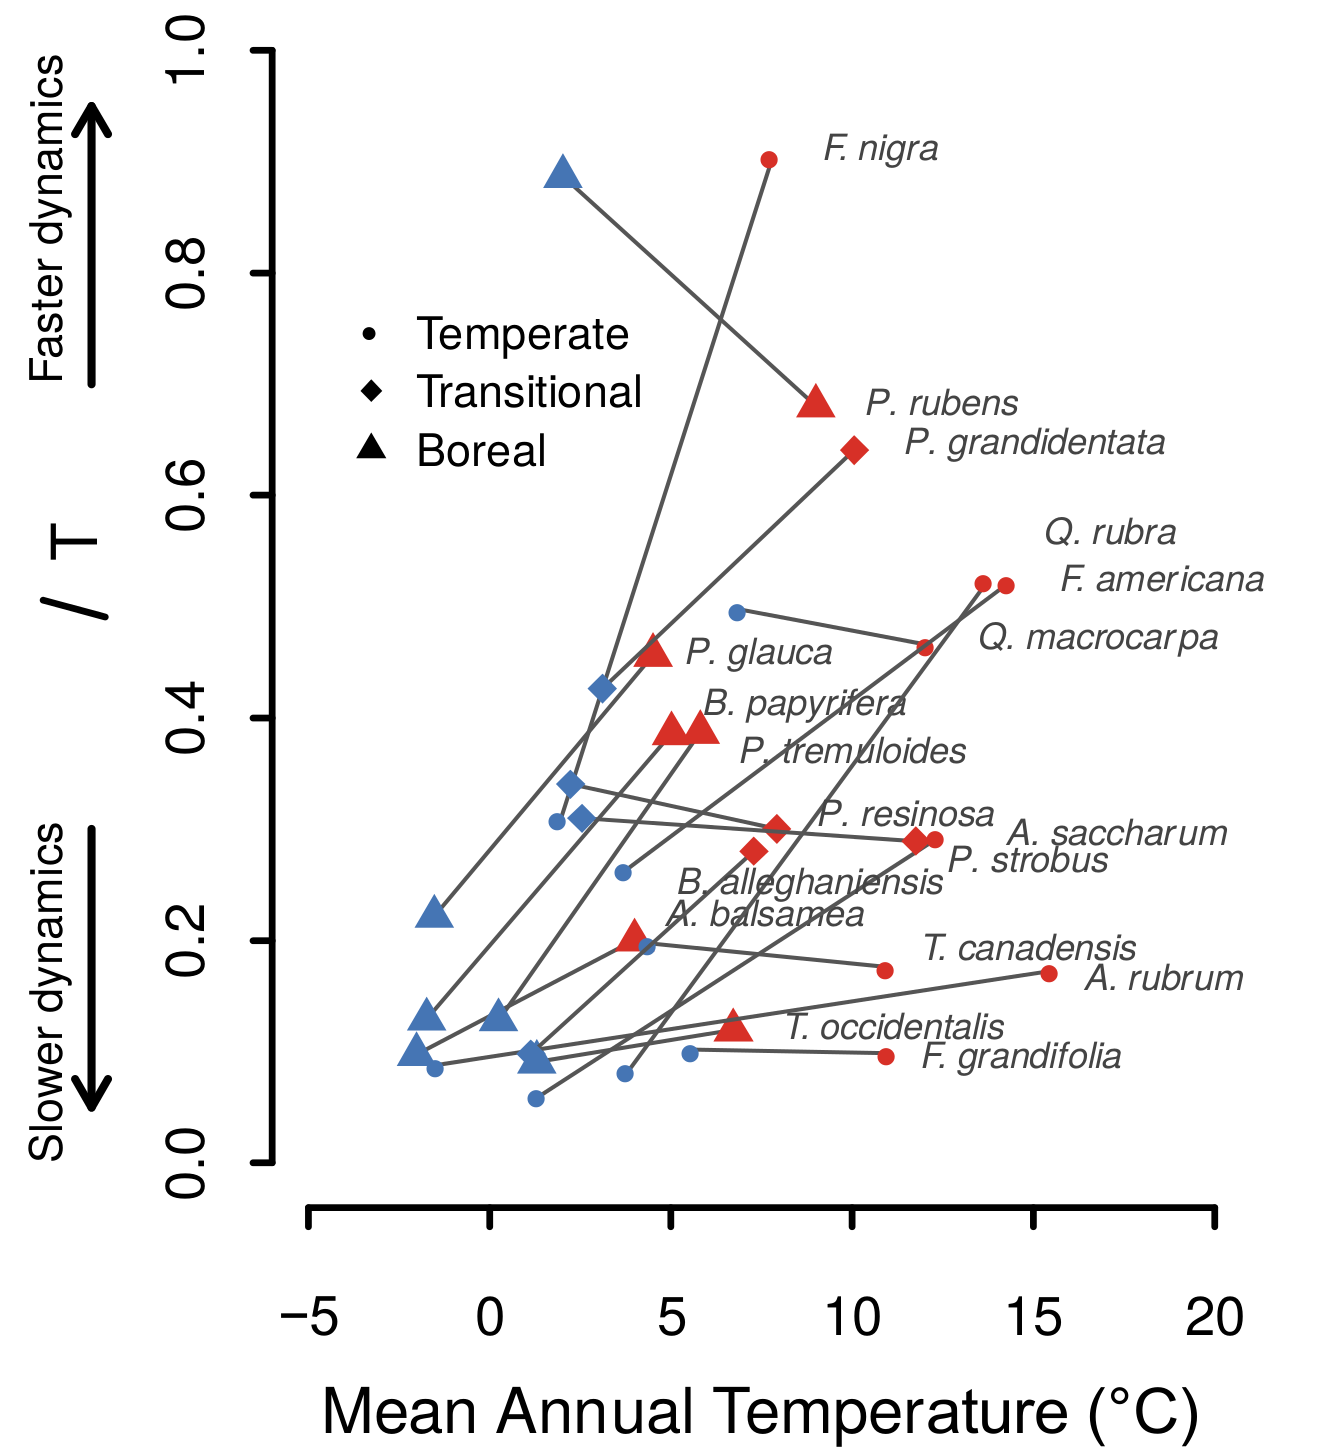
\includegraphics[height=0.55\textheight]{Figs/responsiveness}\\
       \footnotesize{Talluto et al. 2017. Nature Ecology and Evolution} 
    \end{center}
 \end{frame}

%-------------------------------------------------------------------------------

\begin{frame}{Discussion}{Relevance of the theory}
    \begin{columns}
       \begin{column}{0.5\textwidth}
          \begin{center}
             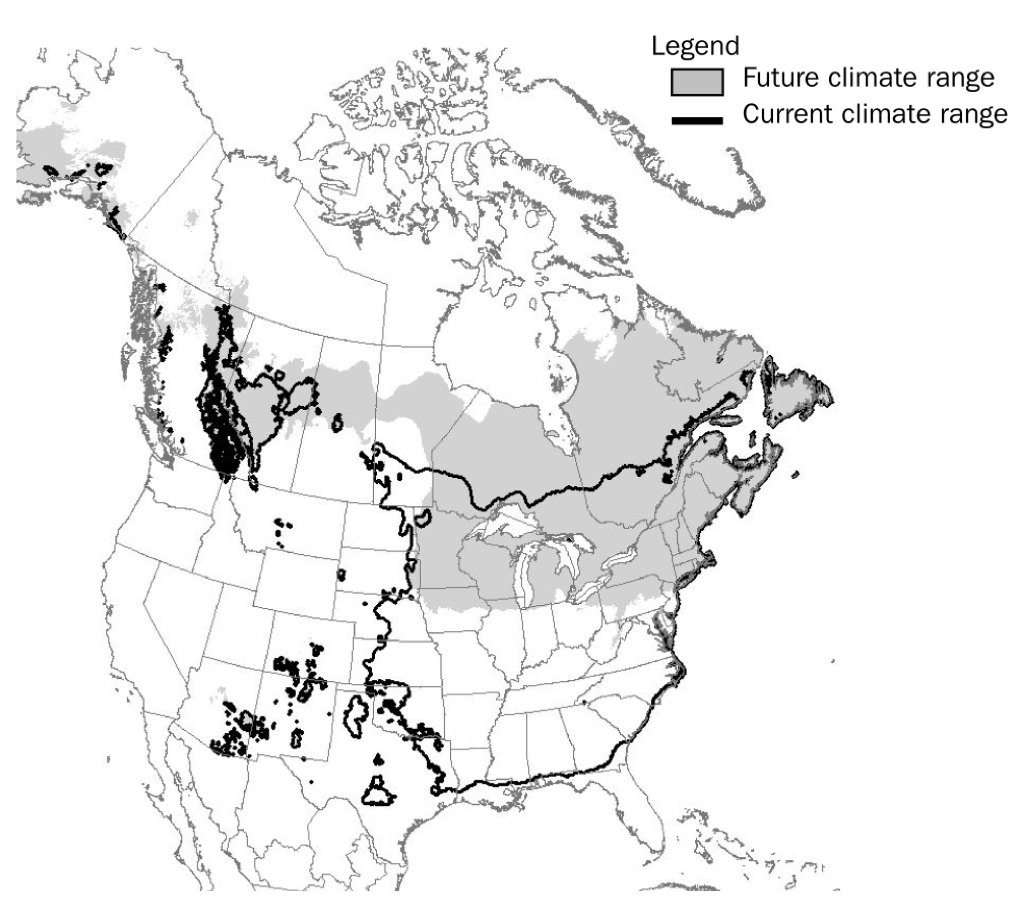
\includegraphics[height=0.5\textheight]{Figs/mckenney}
          \end{center}
       \end{column}
%----
       \begin{column}{0.5\textwidth}
          \begin{itemize}    
             \item A regional perspective on range limits appears to be more appropriate for forest ecosystems;
             \item The framework better accounts for transients;
             \item Many components of the response to climate change;
             \item The statistical approach solves several limitations of SDMs;    
          \end{itemize}
       \end{column}
    \end{columns}        
 \end{frame}

%------------------------------

{
\usebackgroundtemplate{}
\begin{frame}

	\pagecolor{BDQC1st}
	\color{white}

	\LARGE{\textit{Final exercise : patch formation}}

\end{frame}
}

%------------------------------

\begin{frame}{Forest fire model}{Algorithm}
    \begin{columns}
        \begin{column}{0.5\textwidth}
           \begin{center}
              
\includegraphics[height=0.4\textheight]{Figs/fire}
           \end{center}
        \end{column}
 %----
        \begin{column}{0.5\textwidth}
            \begin{itemize}
              \item A burning cell turns into an empty cell
              \item A tree will burn if at least one neighbor is burning
              \item A tree ignites with probability $f$ even if no neighbor is burning
              \item An empty space fills with a tree with probability $p$
           \end{itemize}
        \end{column}
     \end{columns}      
 \end{frame}

%------------------------------
%------------------------------
%------------------------------
\end{document}
